% =============================================================================
% Kapitel 3: Stand der Technik / Verwandte Arbeiten
% -----------------------------------------------------------------------------
% Gliederung:
%  3.1 Klassische Fokuskriterien (Bildschärfe der Rekonstruktion)
%  3.2 Modellbasierter Autofokus für die NFH (Dora et al. 2025, HoloWizard)
%  3.3 Lernbasierter Autofokus in der digitalen Holographie (DH/DHM/DLHM)
%  3.4 Spektrale Parameterschätzung: Analogie zur Kryo-EM (CTFFIND4)
%  3.5 Deep Learning für Phase Retrieval und Holographie, Sim-to-real
%  3.6 Unsicherheit und simulationsbasierte Inferenz in der Bildgebung
%  3.7 Forschungslücke und Abgrenzung (Vergleichstabelle)
% Quellen: ausschließlich die in docs/02_literatur.md verifizierten Arbeiten;
% Zahlenangaben stammen aus den dort dokumentierten Volltexten. Offene Punkte
% sind als "% TODO: mit Betreuern klären" markiert.
% =============================================================================
\chapter{\lang{Stand der Technik}{State of the Art}}
\label{ch:stand}

% Spaltentyp für Tabellen mit Fließtext: linksbündig, feste Breite (array-Paket).
\ifcsname NC@find@L\endcsname\else
  \newcolumntype{L}[1]{>{\raggedright\arraybackslash}p{#1}}
\fi

Dieses Kapitel ordnet die Arbeit in drei Literaturstränge ein. Der erste
Strang behandelt die Autofokussierung in der Holographie: klassische
Fokuskriterien, die die Schärfe einer Rekonstruktion bewerten
(\cref{sec:stand:autofokus}), der modellbasierte Autofokus für die
\ac{nfh}, der den Stand der Technik an der \ac{p05} bildet
(\cref{sec:stand:modellbasiert}), und lernbasierte Verfahren aus der
optischen \ac{dh} (\cref{sec:stand:dl-autofokus}). Der zweite Strang
umfasst Verfahren, die Aufnahmeparameter aus dem Leistungsspektrum schätzen
(\cref{sec:stand:spektral}), sowie den Einsatz von Deep Learning für das
\ac{pr} und die damit verbundene Sim-to-real-Problematik
(\cref{sec:stand:dl-pr}). Der dritte Strang betrifft die Quantifizierung
von Unsicherheiten und die \ac{sbi} in der Bildgebung
(\cref{sec:stand:unsicherheit}). \Cref{sec:stand:abgrenzung} leitet daraus
die Forschungslücke ab und grenzt den Beitrag dieser Arbeit ab.

% -----------------------------------------------------------------------------
\section{\lang{Klassische Fokuskriterien}{Classical Focus Criteria}}
\label{sec:stand:autofokus}
\label{sec:stand:kriterien}

In der digitalen Holographie wird das Objekt numerisch aus dem Hologramm
rückpropagiert; der dafür benötigte Rekonstruktionsabstand ist häufig nur
ungenau bekannt. Das klassische Vorgehen bestimmt ihn durch eine Suche: Für
eine Reihe von Kandidatenabständen wird rekonstruiert, jede Rekonstruktion
mit einem skalaren Schärfemaß bewertet, und der Abstand mit extremalem
Schärfemaß gilt als Fokus. Die Literatur zu solchen Kriterien ist umfangreich;
die für diese Arbeit relevanten Primärquellen sind diejenigen, die
Dora et al.\ \cite{dora2025autofocus} für den Vergleich in der \ac{nfh}
herangezogen haben.

Dubois et al.\ \cite{dubois2006focus} zeigen für die \ac{dhm}, dass der integrierte
Amplitudenbetrag der rekonstruierten Welle im Fokus für reine
Amplitudenobjekte minimal und für reine Phasenobjekte maximal wird, und
leiten daraus ein Fokuskriterium ab. Langehanenberg et al.\
\cite{langehanenberg2008autofocusing} untersuchen für reine Phasenobjekte in der Lebendzellmikroskopie vier
Kriterien, deren Bezeichnungen sich in der Folge etabliert haben: die
gewichtete Spektralanalyse (SPEC), die Bildvarianz (VAR) sowie Statistiken
des Gradienten erster (GRA) und zweiter Ordnung (LAP, Laplace-Operator).
Memmolo et al.\ \cite{memmolo2011automatic} führen den Tamura-Koeffizienten als Maß für die
Sparsity einer Rekonstruktion ein und wenden ihn auch auf gestreckte
Hologramme an. Zhang et al.\ \cite{zhang2017edge} verallgemeinern diesen Gedanken zu
Kantensparsity-Kriterien, die den Tamura-Koeffizienten (ToG) beziehungsweise
den Gini-Index (GoG) auf den Gradientenbetrag der Rekonstruktion anwenden und
dadurch für Amplituden- wie Phasenobjekte dieselbe Peakrichtung besitzen.
Vergleichende Untersuchungen mehrerer Kriterien finden sich für die
In-line-Phasenschiebe-Holographie bei Fonseca et al.\ \cite{fonseca2016comparative}
und im Kontext der holographischen 3D-Partikelverfolgung in der
Übersichtsarbeit von Memmolo et al.\ \cite{memmolo2015recent}.

\begin{table}[tb]
  \centering
  \small
  \caption[Klassische Fokuskriterien und ihr Verhalten in der NFH]{%
    Klassische Fokuskriterien, wie sie Dora et al.\ \cite{dora2025autofocus} in
    der \ac{nfh} untersucht haben. Die Definitionen folgen der Implementierung in HoloWizard
    \cite{dora2026holowizard} (Modul \texttt{core.find\_focus.focus\_loss\_metrics});
    $x$ bezeichnet die rekonstruierte Phase, $g = \abs{\nabla x}$ den
    Gradientenbetrag, $\Delta x$ den diskreten Laplace-Operator und $g_{(k)}$
    die aufsteigend sortierten Werte von $g$. Das Verhalten ist aus den
    Simulations- und Messdatenexperimenten in \cite{dora2025autofocus}
    zusammengefasst.}
  \label{tab:stand:kriterien}
  \begin{tabular}{@{}l L{4.4cm} l L{5.6cm}@{}}
    \toprule
    Kriterium & Definition & Quelle & Verhalten in der \acs{nfh} \cite{dora2025autofocus} \\
    \midrule
    VAR  & $\operatorname{Var}(x)$ & \cite{langehanenberg2008autofocusing} & glatt, aber ohne ausgeprägten Peak; nur rauschrobust \\
    \addlinespace
    SPEC & $\sum \ln\big(1 + \abs{\mathcal{F}[x]}\big)$ ohne Gleichanteil & \cite{langehanenberg2008autofocusing} & verrauscht, plötzliche Peaks, Peakrichtung wechselt je Objekt \\
    \addlinespace
    GRA  & $\sum g$ & \cite{langehanenberg2008autofocusing} & v-förmig in der Simulation; Nebenpeaks auf Messdaten \\
    \addlinespace
    LAP  & $\sum (\Delta x)^2$ & \cite{langehanenberg2008autofocusing} & scharfer, abrupt auftretender Peak; stark rauschempfindlich \\
    \addlinespace
    ToG  & $\sqrt{\operatorname{Var}(g)/\overline{g}}$ & \cite{memmolo2011automatic,zhang2017edge} & v-förmig in der Simulation; Nebenpeaks auf Messdaten \\
    \addlinespace
    GoG  & $1 - 2\sum_{k=1}^{N} \dfrac{g_{(k)}}{\norm{g}_1}\,\dfrac{N - k + \frac12}{N}$ & \cite{zhang2017edge} & wie ToG \\
    \bottomrule
  \end{tabular}
\end{table}
% TODO: mit Betreuern klären, ob die Zuordnung der Primärquellen zu den sechs
%       Kriterien der Referenzliste in Dora et al. 2025 entspricht (die
%       Originalarbeiten wurden hier nur über Titel/Abstract und DOI geprüft).

\Cref{tab:stand:kriterien} fasst die sechs Kriterien zusammen, die in
HoloWizard implementiert sind und die \cite{dora2025autofocus} auf
\ac{nfh}-Daten untersucht haben. Allen gemeinsam ist, dass sie
ausschließlich das rekonstruierte Bild bewerten. In der optischen
Holographie ist das unproblematisch, weil die Rückpropagation eine lineare
Operation ist, die für jeden Kandidatenabstand als \ac{fft} ausgewertet
werden kann. In der \ac{nfh} mit stark wechselwirkenden Objekten ist die
Rekonstruktion dagegen selbst ein nichtlineares, regularisiertes
\ac{pr}-Problem (\cref{sec:grundlagen:pr}), das für jeden Kandidatenabstand
hunderte Iterationen benötigt. Die Fokuskurve ist dann das Ergebnis zweier
gekoppelter Optimierungen, und Artefakte der inneren Rekonstruktion
schlagen auf das Kriterium durch. Dora et al.\ \cite{dora2025autofocus}
formulieren vier
Anforderungen an ein Kriterium, damit ein lokaler Optimierer es zuverlässig
minimieren kann (deutlicher Peak, konsistente Peakrichtung, v- oder
u-förmiger Verlauf über das gesamte Unsicherheitsintervall, Glattheit;
\cref{sec:grundlagen:autofokus}), und zeigen in Simulationen mit drei
Phantomen an 201 Stützstellen sowie auf fünf Messdatensätzen der \ac{p05},
dass keines der sechs Bildkriterien alle Anforderungen erfüllt: VAR besitzt
keinen Peak, SPEC und LAP sind verrauscht beziehungsweise sprunghaft, und
die in der Simulation v-förmigen Kriterien GRA, ToG und GoG zeigen auf
Messdaten Nebenpeaks, in denen ein lokaler Optimierer stecken bleibt.

% -----------------------------------------------------------------------------
\section{\lang{Modellbasierter Autofokus für die Nahfeldholographie}{Model-based Autofocus for Near-field Holography}}
\label{sec:stand:modellbasiert}

\subsection{Das Verfahren von Dora et al.}

Der Stand der Technik für die \ac{nfh} an der \ac{p05} ist der
modellbasierte Autofokus von Dora et al.\ \cite{dora2025autofocus}. Er behandelt das
Problem als geschachtelte Optimierung (\cref{eq:grundlagen:geschachtelt}):
Für einen hypothetischen Abstand $\hat z_{01}$ wird mit der \ac{asrm}
\cite{dora2024asrm} rekonstruiert, und ein äußerer Optimierer sucht den
Abstand, der ein Kriterium $G$ minimiert. Der entscheidende Beitrag ist das
Kriterium selbst: Anstelle einer Bildstatistik misst der \ac{mfe}
(\cref{eq:grundlagen:mfe}) die Konsistenz zwischen Vorwärtsmodell,
Rekonstruktion und Messung. Eine mit falschem Abstand rekonstruierte Welle
enthält Fresnel-Säume mit Werten außerhalb der physikalischen
Nebenbedingungsmenge $\Omega_P$ (positive Phase, Amplituden über eins); die
Projektion auf $\Omega_P$ entfernt diese Werte, und die anschließend zum
Detektor propagierte Welle passt nicht mehr zum gemessenen Hologramm. Der
\ac{mfe} ist damit genau dann minimal, wenn Rekonstruktion und
Vorwärtsmodell das Hologramm gemeinsam erklären. Da die Projektion Teil des
Rekonstruktionsalgorithmus ist, ist der \ac{mfe} ausdrücklich
algorithmusabhängig; in der Praxis entspricht er dem Datenterm der
\ac{asrm}-Rekonstruktion nach der letzten Iteration
\cite{dora2025autofocus}.

Als äußerer Optimierer dient das gradientenfreie Simplexverfahren von
\cite{neldermead1965simplex}. Der Simplex wird mit den beiden Enden des
Unsicherheitsintervalls $\Omega_z = [z^{\mathrm{est}}_{01} - \Delta_M,\
z^{\mathrm{est}}_{01} + \Delta_M]$ initialisiert, Eckpunkte außerhalb des
Intervalls werden auf dessen Rand projiziert, und die Suche endet, sobald
der Simplex kürzer als \qty{100}{\micro\metre} ist. Für die \ac{p05} geben
Dora et al.\ \cite{dora2025autofocus} die Messunsicherheit von $\zOne$ mit
$\Delta_M = \pm\qty{5}{\milli\metre}$ an und zeigen, dass ein Fehler dieser
Größe in $\zOne$ die Fresnel-Zahl signifikant verändert, während derselbe
Fehler in $\zTwo$ vernachlässigbar ist (vgl.\
\cref{fig:grundlagen:sensitivitaet}). Jede Auswertung des Kriteriums ist
eine vollständige Multigrid-Rekonstruktion mit 700, 300 und 500 Iterationen
auf 16-, 4- und 4-fach heruntergetasteten Gittern.
\Cref{fig:stand:autofokus-schema}\,(a) zeigt die Schleife schematisch.

% ---------------------------------------------------------------------------
% Quelle der Abbildung:
%   Skript:  thesis/figures/scripts/autofokus_schema.py (Schema, keine Daten)
%   Aufruf:  /tmp/holo311/bin/python thesis/figures/scripts/autofokus_schema.py
%   Basis:   Commit 36d16b8 (Branch cursor/thesis-grundlagen-6175), 2026-10-01
%   Dateien: autofokus_schema.pdf
% Einbinden im Kapitel: % ---------------------------------------------------------------------------
% Quelle der Abbildung:
%   Skript:  thesis/figures/scripts/autofokus_schema.py (Schema, keine Daten)
%   Aufruf:  /tmp/holo311/bin/python thesis/figures/scripts/autofokus_schema.py
%   Basis:   Commit 36d16b8 (Branch cursor/thesis-grundlagen-6175), 2026-10-01
%   Dateien: autofokus_schema.pdf
% Einbinden im Kapitel: % ---------------------------------------------------------------------------
% Quelle der Abbildung:
%   Skript:  thesis/figures/scripts/autofokus_schema.py (Schema, keine Daten)
%   Aufruf:  /tmp/holo311/bin/python thesis/figures/scripts/autofokus_schema.py
%   Basis:   Commit 36d16b8 (Branch cursor/thesis-grundlagen-6175), 2026-10-01
%   Dateien: autofokus_schema.pdf
% Einbinden im Kapitel: \input{figures/stand_der_technik/autofokus_schema}
% ---------------------------------------------------------------------------
\begin{figure}[tb]
  \centering
  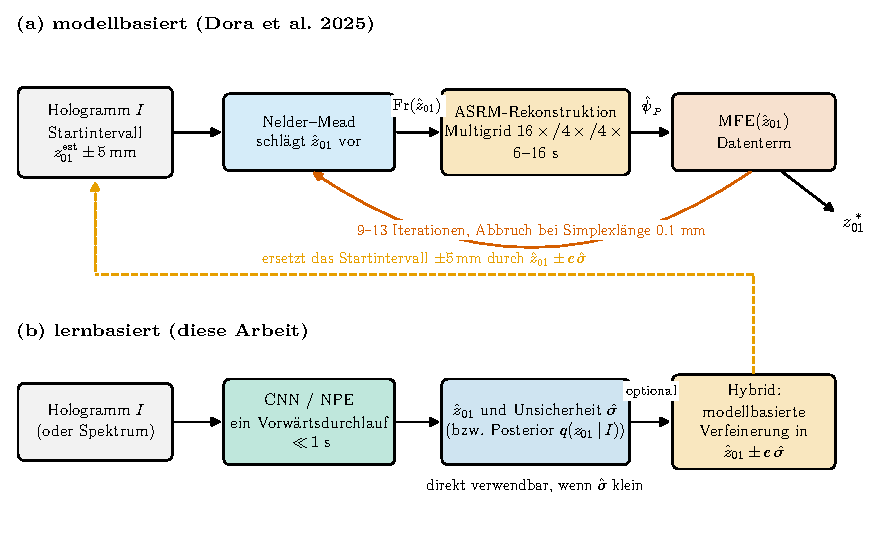
\includegraphics[width=\textwidth]{figures/stand_der_technik/autofokus_schema}
  \caption[Modellbasierter Autofokus und lernbasierte Schätzung im Vergleich]{%
    (a)~Geschachtelte Schleife des modellbasierten Autofokus nach
    \cite{dora2025autofocus}: Der Nelder--Mead-Optimierer schlägt einen Abstand
    $\hat z_{01}$ im Startintervall $z^{\mathrm{est}}_{01} \pm \qty{5}{\milli\metre}$
    vor, eine \ac{asrm}-Rekonstruktion mit der zugehörigen Fresnel-Zahl liefert
    die projizierte Welle $\hat\psi_P$, und der \ac{mfe} bewertet deren
    Konsistenz mit dem Hologramm. Bis zum Abbruch bei einer Simplexlänge von
    \qty{0.1}{\milli\metre} sind 9 bis 13 Rekonstruktionen zu je
    \qtyrange{6}{16}{\second} nötig. (b)~Lernbasierte Schätzung in dieser
    Arbeit: Ein Netz bildet das Hologramm (oder sein Leistungsspektrum) in einem
    Vorwärtsdurchlauf auf eine Schätzung mit Unsicherheit ab; diese ist entweder
    direkt verwendbar oder verengt als Startintervall die modellbasierte
    Verfeinerung (Hybrid).}
  \label{fig:stand:autofokus-schema}
\end{figure}

% ---------------------------------------------------------------------------
\begin{figure}[tb]
  \centering
  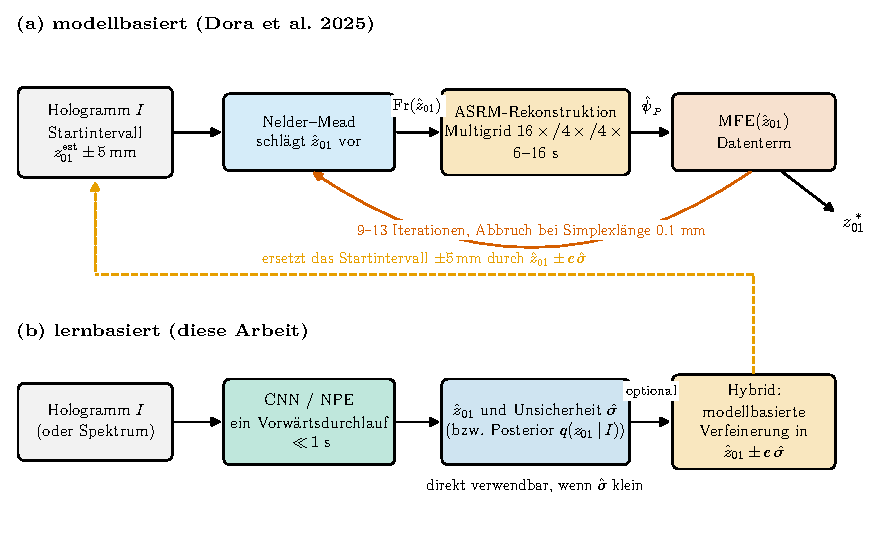
\includegraphics[width=\textwidth]{figures/stand_der_technik/autofokus_schema}
  \caption[Modellbasierter Autofokus und lernbasierte Schätzung im Vergleich]{%
    (a)~Geschachtelte Schleife des modellbasierten Autofokus nach
    \cite{dora2025autofocus}: Der Nelder--Mead-Optimierer schlägt einen Abstand
    $\hat z_{01}$ im Startintervall $z^{\mathrm{est}}_{01} \pm \qty{5}{\milli\metre}$
    vor, eine \ac{asrm}-Rekonstruktion mit der zugehörigen Fresnel-Zahl liefert
    die projizierte Welle $\hat\psi_P$, und der \ac{mfe} bewertet deren
    Konsistenz mit dem Hologramm. Bis zum Abbruch bei einer Simplexlänge von
    \qty{0.1}{\milli\metre} sind 9 bis 13 Rekonstruktionen zu je
    \qtyrange{6}{16}{\second} nötig. (b)~Lernbasierte Schätzung in dieser
    Arbeit: Ein Netz bildet das Hologramm (oder sein Leistungsspektrum) in einem
    Vorwärtsdurchlauf auf eine Schätzung mit Unsicherheit ab; diese ist entweder
    direkt verwendbar oder verengt als Startintervall die modellbasierte
    Verfeinerung (Hybrid).}
  \label{fig:stand:autofokus-schema}
\end{figure}

% ---------------------------------------------------------------------------
\begin{figure}[tb]
  \centering
  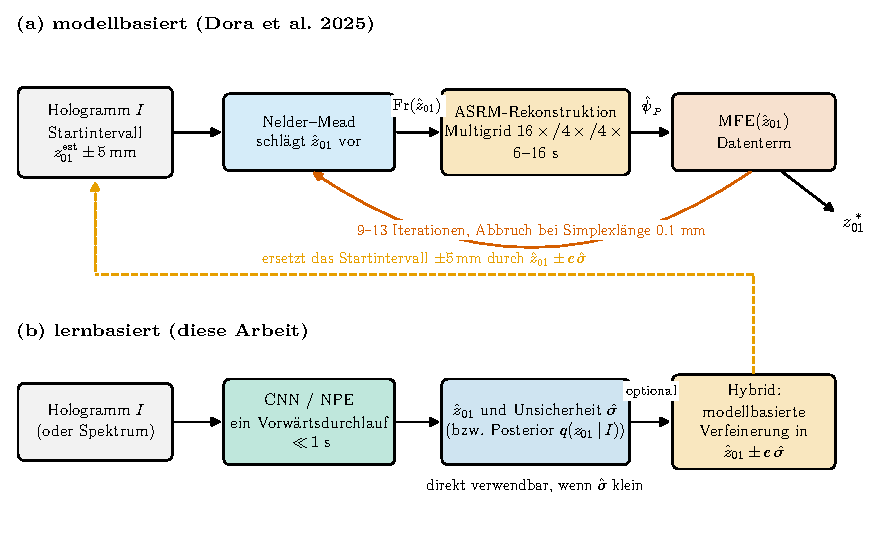
\includegraphics[width=\textwidth]{figures/stand_der_technik/autofokus_schema}
  \caption[Modellbasierter Autofokus und lernbasierte Schätzung im Vergleich]{%
    (a)~Geschachtelte Schleife des modellbasierten Autofokus nach
    \cite{dora2025autofocus}: Der Nelder--Mead-Optimierer schlägt einen Abstand
    $\hat z_{01}$ im Startintervall $z^{\mathrm{est}}_{01} \pm \qty{5}{\milli\metre}$
    vor, eine \ac{asrm}-Rekonstruktion mit der zugehörigen Fresnel-Zahl liefert
    die projizierte Welle $\hat\psi_P$, und der \ac{mfe} bewertet deren
    Konsistenz mit dem Hologramm. Bis zum Abbruch bei einer Simplexlänge von
    \qty{0.1}{\milli\metre} sind 9 bis 13 Rekonstruktionen zu je
    \qtyrange{6}{16}{\second} nötig. (b)~Lernbasierte Schätzung in dieser
    Arbeit: Ein Netz bildet das Hologramm (oder sein Leistungsspektrum) in einem
    Vorwärtsdurchlauf auf eine Schätzung mit Unsicherheit ab; diese ist entweder
    direkt verwendbar oder verengt als Startintervall die modellbasierte
    Verfeinerung (Hybrid).}
  \label{fig:stand:autofokus-schema}
\end{figure}


\subsection{Ergebnisse und Kennzahlen}

In einer rauschfreien Simulation mit drei Phantomen an 201 Stützstellen
verlaufen \ac{mfe}, GRA, GoG und ToG v-förmig, VAR besitzt keinen Peak, und
LAP sowie SPEC sind verrauscht beziehungsweise inkonsistent. Auf den fünf
Messdatensätzen der \ac{p05} (\cref{tab:stand:dora-objekte}) zeigen alle
Bildkriterien Nebenpeaks oder keinen Peak, der \ac{mfe} dagegen nur
\enquote{minor saddle points} \cite{dora2025autofocus}. Im Autofokus-Testlauf
konvergiert das Verfahren bei allen fünf Objekten bis auf höchstens
\qty{0.1}{\milli\metre} auf den visuell bestimmten Referenzabstand und
benötigt dafür 9 bis 13 Probepunkte. Eine Rekonstruktion dauert \qty{6}{\second}
auf einem Gitter von $8192^2$ Pixeln beziehungsweise \qty{16}{\second} bei
$14\,336^2$ Pixeln (jeweils gepaddet und für die letzte Stufe vierfach
heruntergetastet), so dass eine Fokussierung insgesamt \enquote{a few
minutes} in Anspruch nimmt. \Cref{tab:stand:dora-kennzahlen} stellt die
Kennzahlen zusammen.
% TODO: mit Betreuern klären, auf welcher Hardware (GPU-Typ) die Zeiten in
%       Dora et al. 2025 gemessen wurden; das Paper nennt sie nicht.

\begin{table}[tb]
  \centering
  \small
  \caption[Messobjekte der Autofokus-Evaluation in Dora et al. 2025]{%
    Messobjekte, mit denen Dora et al.\ \cite{dora2025autofocus} den
    modellbasierten Autofokus an der \ac{p05} evaluieren (Tab.~2 dort). Die Fresnel-Zahlen
    sind die im Paper angegebenen Werte; alle Aufnahmen verwenden
    $\dx = \qty{6.5}{\micro\metre}$ und $\zTwo$ zwischen \qty{19.65}{\metre}
    und \qty{19.91}{\metre}.}
  \label{tab:stand:dora-objekte}
  \begin{tabular}{@{}l S[table-format=2.0] S[table-format=3.1] S[table-format=2.3] l@{}}
    \toprule
    Objekt & {$E$ in \unit{\kilo\electronvolt}} & {$\zOne$ in \unit{\milli\metre}} & {$\zTwo$ in \unit{\metre}} & $\Fr$ (Paper) \\
    \midrule
    Spinnenhaar               & 11 &  79.4 & 19.661 & \num{7.79e-5} \\
    Zahn                      & 17 &  81.0 & {--}   & -- \\
    Kaktusnadel               & 17 & 284.1 & {--}   & -- \\
    Magnesiumdraht            & 11 & 470.8 & 19.661 & \num{4.678e-4} \\
    Magnesiumdraht, Flusszelle & 11 & 329.3 & 19.914 & \num{3.165e-4} \\
    \bottomrule
  \end{tabular}
\end{table}
% TODO: mit Betreuern klären bzw. aus Tab. 2 in Dora et al. 2025 ergänzen:
%       z02 und Fr für Zahn und Kaktusnadel (in den Projektnotizen nur der
%       Gesamtbereich 7.8e-5 bis 4.7e-4 bzw. 19.65-19.91 m notiert).

\begin{table}[tb]
  \centering
  \caption[Kennzahlen des modellbasierten Autofokus]{%
    Kennzahlen des modellbasierten Autofokus nach \cite{dora2025autofocus}
    und ihre Entsprechung in HoloWizard \cite{dora2026holowizard}.}
  \label{tab:stand:dora-kennzahlen}
  \footnotesize
  \begin{tabular}{@{}L{3.0cm} L{6.2cm} L{4.5cm}@{}}
    \toprule
    Größe & Wert & HoloWizard \\
    \midrule
    Unsicherheitsintervall $\Delta_M$ & $\pm\qty{5}{\milli\metre}$ um $z^{\mathrm{est}}_{01}$ & \texttt{Measurement}, Feld \texttt{z01\_confidence} \\
    \addlinespace
    Optimierer & Nelder--Mead, Simplex an den Intervallenden, Projektion auf $\Omega_z$ & \texttt{scipy}, Methode \texttt{Nelder-Mead}, \texttt{initial\_simplex} \\
    \addlinespace
    Abbruchkriterium & Simplexlänge $< \qty{100}{\micro\metre}$ & \texttt{Options}, Feld \texttt{z01\_tol} $= \qty{0.1}{\milli\metre}$ (\texttt{xatol}) \\
    \addlinespace
    Fokuskriterium & \acs{mfe}, Datenterm nach der letzten Iteration & \texttt{loss\_se\_all[-1]} \\
    \addlinespace
    Innerer Löser & \acs{asrm}, Multigrid 700/300/500 Iterationen bei $16\times$/$4\times$/$4\times$ & \texttt{reconstruct\_multistage} \\
    \addlinespace
    Probepunkte je Datensatz & 9 bis 13 Rekonstruktionen & -- \\
    \addlinespace
    Dauer je Rekonstruktion & \qty{6}{\second} ($8192^2$ Pixel) bzw.\ \qty{16}{\second} ($14\,336^2$ Pixel) & -- \\
    \addlinespace
    Gesamtdauer & \enquote{a few minutes} & -- \\
    \addlinespace
    Genauigkeit & $\le \qty{0.1}{\milli\metre}$ gegenüber visueller Referenz (fünf Objekte) & -- \\
    \addlinespace
    Hardware & nicht angegeben & -- \\
    \bottomrule
  \end{tabular}
\end{table}

\subsection{Implementierung in HoloWizard und Livereco}

Das Verfahren ist im Python-Framework HoloWizard
\cite{dora2024framework,dora2026holowizard} implementiert. Die öffentliche
Funktion \texttt{find\_focus} im Paket \texttt{core.api} lädt das Hologramm,
bildet die Amplitude $\sqrt{I}$ und ruft die eindimensionale Suche im Paket
\texttt{core.find\_focus} auf. Diese verwendet
\texttt{scipy.optimize.minimize} mit der Methode \texttt{Nelder-Mead}, dem
Startsimplex aus den Intervallgrenzen und der Toleranz \texttt{xatol}
$= \qty{0.1}{\milli\metre}$; die Zielfunktion setzt $\zOne$ in der
Messbeschreibung, startet die Multigrid-Rekonstruktion und gibt den
Datenterm der letzten Stufe zurück. Die Parameterobjekte
\texttt{Measurement} (Felder \texttt{z01}, \texttt{z01\_confidence}) und
\texttt{Options} (Feld \texttt{z01\_tol}) kapseln Startschätzung,
Intervallbreite (Standard \qty{5}{\milli\metre}) und Abbruchtoleranz; die
Klasse \texttt{ConeBeam} rechnet die Geometrie nach
\cref{eq:grundlagen:fresnelzahl} und \cref{eq:grundlagen:z01-aus-fr} um.
Über das Paper hinaus enthält der Code eine gemeinsame Suche über $\zOne$
und den Intensitätsoffset $a_0$ (auch als orthogonale Suche), eine Variante
mit Flatfield-Korrektur sowie die klassischen Kriterien aus
\cref{tab:stand:kriterien} für Fokusserien. Für den Beamline-Betrieb ist
die Suche im Livereco-Server (Paket \texttt{livereco}) und in der
Pipeline-Schnittstelle (Paket \texttt{pipe}) gekapselt. Die Integration
eines lernbasierten Schätzers kann daher ohne Änderung des Pakets über die
bestehende Schnittstelle erfolgen, indem Startwert und Intervallbreite
gesetzt werden.

\subsection{Grenzen}

Aus der Arbeit von Dora et al.\ \cite{dora2025autofocus} und der
Implementierung ergeben sich die folgenden Grenzen, die diese Arbeit adressiert oder zumindest berührt:
\begin{enumerate}
  \item \emph{Laufzeit}: Jede Fokussierung erfordert 9 bis 13 vollständige
    Rekonstruktionen und dauert Minuten. Für die Online-Rekonstruktion,
    Tomographie-Serien mit Driften oder In-situ-Experimente, bei denen sich
    $\zOne$ häufig ändert, ist das ein Engpass.
  \item \emph{Lokalität}: Nelder--Mead ist ein lokaler Optimierer, der eine
    v- oder u-förmige Fokuskurve innerhalb von $\Omega_z$ und eine
    Startschätzung innerhalb $\pm\Delta_M$ voraussetzt.
  \item \emph{Abhängigkeit von Hyperparametern}: Das Ergebnis hängt von den
    Einstellungen der \ac{asrm}, dem Offset $A_0$ und dem Padding ab.
  \item \emph{Evaluationsumfang}: fünf Messobjekte und drei Phantome; die
    Simulation ist rauschfrei und ohne Flatfield-Artefakte.
  \item \emph{Nur $\zOne$}: $\zTwo$, $E$ und $\dx$ gelten als bekannt; eine
    Erweiterung auf weitere Parameter wird als möglich bezeichnet.
  \item \emph{Keine Unsicherheitsangabe}: Das Verfahren liefert einen
    Punktwert, aber kein Maß dafür, wie verlässlich er ist.
  \item \emph{Referenz}: Die Referenzabstände sind visuell bestimmt; eine
    unabhängige Grundwahrheit existiert für Messdaten nicht.
\end{enumerate}
Insbesondere die Laufzeit motiviert einen Schätzer, der ohne Rekonstruktion
auskommt, und das Fehlen einer Unsicherheit motiviert die probabilistischen
Varianten in \cref{sec:stand:unsicherheit}.

% -----------------------------------------------------------------------------
\section{\lang{Lernbasierter Autofokus in der digitalen Holographie}{Learning-based Autofocus in Digital Holography}}
\label{sec:stand:dl-autofokus}

Lernbasierte Autofokusverfahren sind bislang ausschließlich für die optische
\ac{dh} und \ac{dhm} mit sichtbarem Licht beschrieben worden. Ihre
gemeinsame Idee ist, die Suche über einen Rekonstruktionsstapel durch eine
einzige Auswertung eines Netzes zu ersetzen, das den Fokusabstand direkt
aus dem Hologramm liest. Nach Rivenson et al.\ \cite{rivenson2019deep} zählen solche
Verfahren zu einer breiteren Entwicklung, in der datengetriebene Modelle
iterative Rekonstruktionsschritte der kohärenten Bildgebung durch
Vorwärtsdurchläufe ersetzen.

Frühe Arbeiten formulierten die Aufgabe als Klassifikation über wenige
diskrete Fokusebenen \cite{pitkaaho2017performance}. Ren et al.\
\cite{ren2018learning} behandeln sie erstmals als Regression: Ein \ac{cnn} bildet das Hologramm
ohne Rekonstruktion und ohne Fokuskriterium auf einen skalaren Abstand ab.
Der Datensatz umfasst zehn Abstände zwischen \qty{250}{\milli\metre} und
\qty{272}{\milli\metre} mit je 500 Hologrammen, also 5000 Hologramme, die
im Verhältnis 75/15/10 aufgeteilt und mit dem Adam-Verfahren trainiert
wurden. Das \ac{cnn} erreicht einen \ac{mae} von etwa \qty{0.05}{\milli\metre}
für Amplitudenobjekte und \qtyrange{0.04}{0.06}{\milli\metre} in weiteren
Experimenten ($R^2 \approx 0.97$), während ein $k$-Nächste-Nachbarn-Regressor
auf handgemachten Merkmalen bei \qtyrange{1.2}{1.6}{\milli\metre} liegt und
Support-Vektor-Regression sowie \ac{mlp} ähnlich schlecht abschneiden. Die
Vorhersage erwies sich als robust gegenüber Belichtungszeiten zwischen
\qty{5}{\milli\second} und \qty{18}{\milli\second}. Zu beachten ist, dass
nur zehn diskrete Abstände vorkommen; eine Generalisierung über ein
kontinuierliches Abstandsintervall wurde nicht untersucht.

Pitkäaho et al.\ \cite{pitkaaho2019focus} setzen vortrainierte Bildklassifikationsnetze
(AlexNet, VGG16) per Transfer Learning für die Fokusprädiktion aus
Off-axis-\ac{dhm}-Hologrammen ein, nach Entfernung der nullten
Beugungsordnung und des Zwillingsbilds. Der RMS-Fehler beträgt
\qty{6.37}{\milli\metre} (AlexNet) beziehungsweise \qty{6.49}{\milli\metre}
(VGG16) bei einer akzeptierten Toleranz von \qty{20}{\milli\metre}, innerhalb
derer nahezu alle Vorhersagen liegen. Der Laufzeitvorteil ist deutlich: Die
Inferenz dauert \qty{247}{\milli\second} beziehungsweise
\qty{680}{\milli\second} auf einer Laptop-CPU ohne \ac{gpu}, gegenüber
\qty{932}{\milli\second} für eine einzige Auswertung des Tamura-Kriteriums
einschließlich Rekonstruktion. Die Genauigkeit im Millimeterbereich liegt
jedoch weit unter den Anforderungen der \ac{nfh}; ein plausibler Grund ist,
dass vortrainierte Netze ihre Eingaben auf eine feste Größe skalieren und
damit die Streifenskala verändern, die die Information über den Abstand
trägt (\cref{sec:grundlagen:dl}).

Jaferzadeh et al.\ \cite{jaferzadeh2019nosearch} prädizieren den Fokus pro Objekt statt pro
Bild: Aus Off-axis-Hologrammen roter Blutkörperchen schätzt ein \ac{cnn}
den Fokusabstand jeder einzelnen Zelle ohne Suche über einen
Rekonstruktionsstapel, bei gegenüber dem Suchverfahren vergleichbarer
Genauigkeit und deutlich geringerer Laufzeit. Die Referenzlabels stammen
dabei aus einem klassischen Fokuskriterium -- ein Vorgehen, das sich auf die
\ac{nfh} übertragen lässt, wo der modellbasierte Autofokus die
Referenzabstände für Messdaten liefert.

Geometrisch am nächsten an der \ac{nfh} liegt FocusNET von
Montoya et al.\ \cite{montoya2023focusnet} für die \acf{dlhm}, die wie die \ac{nfh} eine
In-line-Kegelstrahlgeometrie mit einer Punktquelle verwendet. Ein \ac{cnn}
regressiert den Rekonstruktionsabstand mit einer Standardabweichung der
Vorhersage von etwa \qty{54}{\micro\metre} und ist etwa 600-mal schneller
als die Fokussuche über einen Rekonstruktionsstapel; der Detektor hat
$3518 \times 3518$ Pixel, so dass große Sensoren patchweise verarbeitet
werden. Diese Arbeit belegt, dass In-line-Hologramme eine Genauigkeit unter
\qty{100}{\micro\metre} zulassen, und etabliert den Laufzeitvergleich
gegenüber einem Suchverfahren als Berichtsgröße.

\begin{table}[tb]
  \centering
  \caption[Lernbasierte Autofokusverfahren in der digitalen Holographie]{%
    Lernbasierte Autofokusverfahren in der optischen Holographie im Vergleich
    zum modellbasierten Verfahren für die \ac{nfh}. Angaben nach den
    jeweiligen Publikationen; \enquote{k.\,A.} bedeutet, dass die Größe dort
    nicht berichtet oder in den ausgewerteten Fassungen nicht enthalten ist.}
  \label{tab:stand:dl-vergleich}
  \footnotesize
  \begin{tabular}{@{}L{1.3cm} L{2.2cm} L{2.6cm} L{4.2cm} L{2.6cm}@{}}
    \toprule
    Arbeit & Modalität & Zielgröße; Formulierung & Daten; Genauigkeit & Laufzeit \\
    \midrule
    \cite{pitkaaho2017performance} & \acs{dhm} & Fokusebene; Klassifikation (\acs{cnn}) & wenige diskrete Ebenen; k.\,A. & k.\,A. \\
    \addlinespace
    \cite{ren2018learning} & \acs{dh}, sichtbar & Abstand; Regression (\acs{cnn}) & 5000 Messhologramme an 10 Abständen; \acs{mae} $\approx \qty{0.05}{\milli\metre}$ & k.\,A. \\
    \addlinespace
    \cite{pitkaaho2019focus} & Off-axis-\acs{dhm} & Abstand; Regression (AlexNet, VGG16, Transfer) & Messhologramme; RMS \qty{6.4}{\milli\metre} bei \qty{20}{\milli\metre} Toleranz & \qtyrange{0.25}{0.68}{\second} je Hologramm (CPU) \\
    \addlinespace
    \cite{jaferzadeh2019nosearch} & Off-axis-\acs{dhm} & Abstand je Zelle; Regression (\acs{cnn}) & Messhologramme, Labels aus Fokuskriterium; vergleichbar mit Suche & schneller als Suche \\
    \addlinespace
    \cite{montoya2023focusnet} & \acs{dlhm}, In-line, Kegelstrahl & Abstand; Regression (\acs{cnn}) & Std.\ der Vorhersage $\approx \qty{54}{\micro\metre}$ & $\approx 600\times$ schneller als Stapelsuche \\
    \midrule
    \cite{dora2025autofocus} & Röntgen-\acs{nfh}, Kegelstrahl & $\zOne$; modellbasierte Optimierung & 5 Messobjekte, 3 Phantome; $\le \qty{0.1}{\milli\metre}$ & Minuten (9 bis 13 Rekonstruktionen) \\
    \bottomrule
  \end{tabular}
\end{table}

\Cref{tab:stand:dl-vergleich} stellt die Arbeiten gegenüber. Für die
Übertragung auf die \ac{nfh} sind fünf Unterschiede wesentlich. Erstens
liegt die Fresnel-Zahl der \ac{nfh} in Pixeleinheiten bei
\numrange{2e-5}{5e-4} (\cref{tab:grundlagen:geometrie}); die
Fresnel-Säume erstrecken sich über hunderte Pixel, und die
Mindestgittergröße $1/\Fr$ übersteigt die typische Detektorgröße. Zweitens
sind die Objekte stark wechselwirkend, so dass die Linearisierung der
\ac{ctf} nicht gilt und keine lineare Rückpropagation als Zwischenschritt
zur Verfügung steht. Drittens muss ein kontinuierliches Intervall
$\zOne \in [\qty{20}{\milli\metre}, \qty{500}{\milli\metre}]$ abgedeckt
werden, nicht wenige diskrete Abstände. Viertens stehen für die \ac{nfh}
keine großen Messdatensätze mit Referenzabständen zur Verfügung; die
Trainingsdaten müssen simuliert werden, womit die Sim-to-real-Lücke
(\cref{sec:stand:dl-pr}) zum zentralen Risiko wird. Fünftens erfordert die
Zielgenauigkeit von \qty{0.1}{\milli\metre} bei $\zOne = \qty{250}{\milli\metre}$
eine relative Genauigkeit von \qty{0.04}{\percent} in $\Fr$
(\cref{eq:grundlagen:fehlerfortpflanzung}) -- eine Größenordnung
anspruchsvoller als die relative Genauigkeit der zitierten optischen
Arbeiten.

% -----------------------------------------------------------------------------
\section{\lang{Spektrale Parameterschätzung: Analogie zur Elektronenmikroskopie}{Spectral Parameter Estimation: Analogy to Electron Microscopy}}
\label{sec:stand:spektral}

Die Bestimmung eines Aufnahmeparameters aus dem Leistungsspektrum eines
Bildes ist in der Kryo-\ac{em} Routine. Dort moduliert die
Kontrastübertragungsfunktion des Mikroskops das Spektrum einer Aufnahme mit
Ringen (Thon-Ringen), deren Lage vom Defokus abhängt. Das Standardwerkzeug
\textsc{CTFFIND4} von Rohou und Grigorieff \cite{rohou2015ctffind4} passt ein \ac{ctf}-Modell der
Form $\sin(\pi\wl\abs{\vect{g}}^2\Delta f - \dots)$ an das Amplitudenspektrum
an, schätzt daraus Defokus und Astigmatismus und gibt ein Gütemaß als
Funktion der Ortsfrequenz aus, das angibt, bis zu welcher Auflösung die
Ringe dem Modell folgen. Das Verfahren ist schnell, benötigt keine
Trainingsdaten und ist unabhängig vom abgebildeten Objekt, solange dessen
Spektrum die betreffenden Frequenzen enthält.

% ---------------------------------------------------------------------------
% Quelle der Abbildung:
%   Skript:  thesis/figures/scripts/hologramm_simulation.py (eigene Fresnel-Simulation,
%            N = 512, Padding 2, kein Trainingslauf, kein HoloForge-Datensatz)
%   Aufruf:  /tmp/holo311/bin/python thesis/figures/scripts/hologramm_simulation.py
%   Basis:   Commit 1abccf9 (Branch cursor/thesis-grundlagen-6175), 2026-10-01
%   Dateien: radialprofil_spektrum.pdf (dasselbe Skript erzeugt
%            figures/grundlagen/hologramm_spektrum.pdf)
% Einbinden im Kapitel: % ---------------------------------------------------------------------------
% Quelle der Abbildung:
%   Skript:  thesis/figures/scripts/hologramm_simulation.py (eigene Fresnel-Simulation,
%            N = 512, Padding 2, kein Trainingslauf, kein HoloForge-Datensatz)
%   Aufruf:  /tmp/holo311/bin/python thesis/figures/scripts/hologramm_simulation.py
%   Basis:   Commit 1abccf9 (Branch cursor/thesis-grundlagen-6175), 2026-10-01
%   Dateien: radialprofil_spektrum.pdf (dasselbe Skript erzeugt
%            figures/grundlagen/hologramm_spektrum.pdf)
% Einbinden im Kapitel: % ---------------------------------------------------------------------------
% Quelle der Abbildung:
%   Skript:  thesis/figures/scripts/hologramm_simulation.py (eigene Fresnel-Simulation,
%            N = 512, Padding 2, kein Trainingslauf, kein HoloForge-Datensatz)
%   Aufruf:  /tmp/holo311/bin/python thesis/figures/scripts/hologramm_simulation.py
%   Basis:   Commit 1abccf9 (Branch cursor/thesis-grundlagen-6175), 2026-10-01
%   Dateien: radialprofil_spektrum.pdf (dasselbe Skript erzeugt
%            figures/grundlagen/hologramm_spektrum.pdf)
% Einbinden im Kapitel: \input{figures/stand_der_technik/radialprofil_spektrum}
% ---------------------------------------------------------------------------
\begin{figure}[tb]
  \centering
  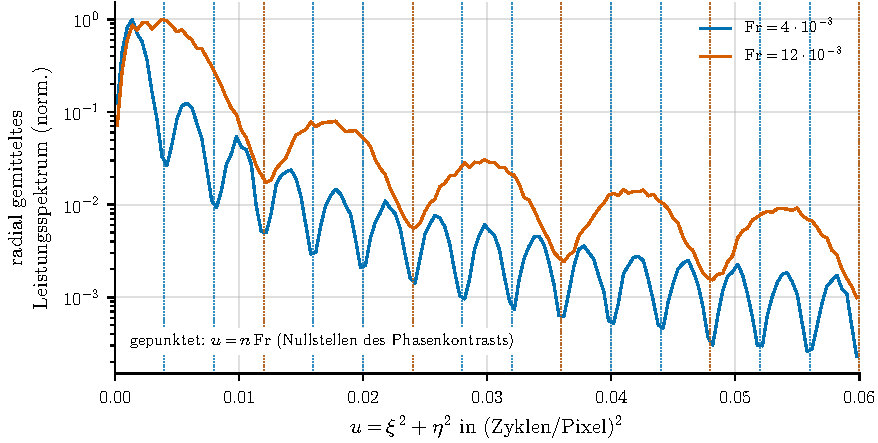
\includegraphics[width=\textwidth]{figures/stand_der_technik/radialprofil_spektrum}
  \caption[Radial gemitteltes Leistungsspektrum simulierter Hologramme über $\xi^2+\eta^2$]{%
    Radial gemitteltes Leistungsspektrum der simulierten Hologramme des schwachen
    Phasenobjekts aus \cref{fig:grundlagen:hologramm}\,(b,\,e), aufgetragen über
    $u = \xi^2+\eta^2$. In dieser Koordinate liegen die Minima
    äquidistant bei $u = n\,\Fr$ (gepunktete Linien), analog zu den Thon-Ringen,
    aus denen \textsc{CTFFIND4} den Defokus elektronenmikroskopischer Aufnahmen
    schätzt \cite{rohou2015ctffind4}. Die Periode des Musters ist unmittelbar die
    Fresnel-Zahl; das Objektspektrum bestimmt nur die Einhüllende.}
  \label{fig:stand:radialprofil}
\end{figure}

% ---------------------------------------------------------------------------
\begin{figure}[tb]
  \centering
  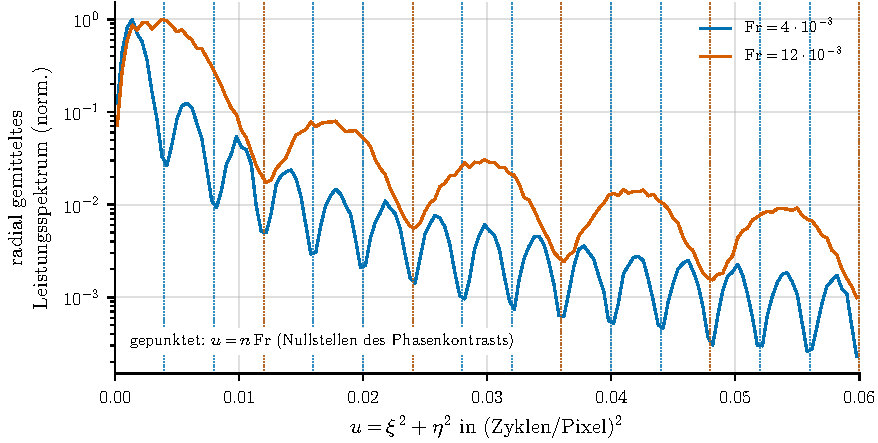
\includegraphics[width=\textwidth]{figures/stand_der_technik/radialprofil_spektrum}
  \caption[Radial gemitteltes Leistungsspektrum simulierter Hologramme über $\xi^2+\eta^2$]{%
    Radial gemitteltes Leistungsspektrum der simulierten Hologramme des schwachen
    Phasenobjekts aus \cref{fig:grundlagen:hologramm}\,(b,\,e), aufgetragen über
    $u = \xi^2+\eta^2$. In dieser Koordinate liegen die Minima
    äquidistant bei $u = n\,\Fr$ (gepunktete Linien), analog zu den Thon-Ringen,
    aus denen \textsc{CTFFIND4} den Defokus elektronenmikroskopischer Aufnahmen
    schätzt \cite{rohou2015ctffind4}. Die Periode des Musters ist unmittelbar die
    Fresnel-Zahl; das Objektspektrum bestimmt nur die Einhüllende.}
  \label{fig:stand:radialprofil}
\end{figure}

% ---------------------------------------------------------------------------
\begin{figure}[tb]
  \centering
  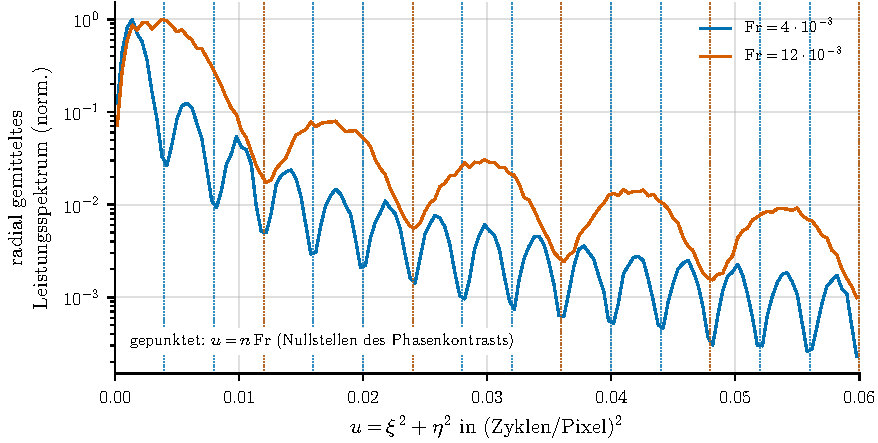
\includegraphics[width=\textwidth]{figures/stand_der_technik/radialprofil_spektrum}
  \caption[Radial gemitteltes Leistungsspektrum simulierter Hologramme über $\xi^2+\eta^2$]{%
    Radial gemitteltes Leistungsspektrum der simulierten Hologramme des schwachen
    Phasenobjekts aus \cref{fig:grundlagen:hologramm}\,(b,\,e), aufgetragen über
    $u = \xi^2+\eta^2$. In dieser Koordinate liegen die Minima
    äquidistant bei $u = n\,\Fr$ (gepunktete Linien), analog zu den Thon-Ringen,
    aus denen \textsc{CTFFIND4} den Defokus elektronenmikroskopischer Aufnahmen
    schätzt \cite{rohou2015ctffind4}. Die Periode des Musters ist unmittelbar die
    Fresnel-Zahl; das Objektspektrum bestimmt nur die Einhüllende.}
  \label{fig:stand:radialprofil}
\end{figure}


Die Analogie zur \ac{nfh} ist unmittelbar: Nach \cref{eq:grundlagen:ctf}
liegen die Nullstellen des Phasenkontrasts bei $\abs{\vect{\xi}}^2 = n\,\Fr$,
und das Leistungsspektrum eines Hologramms trägt dieselbe Ringsignatur mit
der Fresnel-Zahl als Periode in der Koordinate $u = \xi^2 + \eta^2$
(\cref{fig:grundlagen:hologramm}). \Cref{fig:stand:radialprofil} zeigt das
radial gemittelte Spektrum simulierter Hologramme eines schwachen
Phasenobjekts: Die Minima liegen äquidistant bei $u = n\,\Fr$, und das
Objektspektrum bestimmt lediglich die Einhüllende. Ein
\textsc{CTFFIND4}-artiger Ringfit -- Radialmittelung, Untergrundabzug,
Anpassung der Periode -- ist damit eine naheliegende, nicht lernbasierte
Referenz für den Autofokus und zugleich die Motivation, das
Leistungsspektrum oder sein Radialprofil als Eingabe eines lernenden
Verfahrens zu verwenden (\cref{ch:methoden}). Gegenüber der Kryo-\ac{em}
bestehen jedoch Unterschiede, die einen reinen Fit erschweren: Die Objekte
der \ac{nfh} sind stark wechselwirkend, so dass die Linearisierung der
\ac{ctf} nur näherungsweise gilt und Absorptions- und Phasenanteil mit
unterschiedlichen Nullstellen überlagern (\cref{eq:grundlagen:ctf-nullstellen});
die strukturierte Beleuchtung und das Flatfield prägen dem Spektrum eigene
Anteile auf; und bei den kleinen Fresnel-Zahlen der \ac{nfh} werden
innerhalb des Nyquist-Bereichs eines $N^2$-Hologramms nur Ringe bis
$u < N\Fr/2$ aufgelöst (\cref{sec:grundlagen:ctf}), so dass bei
$\Fr \approx \num{1e-4}$ und $N = 2048$ nur wenige zehn Ringe zur
Verfügung stehen. Eine Anwendung spektraler Fits auf den Autofokus der
\ac{nfh} ist in der ausgewerteten Literatur nicht beschrieben.

% -----------------------------------------------------------------------------
\section{\lang{Deep Learning für Phase Retrieval und Holographie}{Deep Learning for Phase Retrieval and Holography}}
\label{sec:stand:dl-pr}

Der Autofokus ist ein Teilproblem der lernbasierten holographischen
Rekonstruktion, die Rivenson et al.\ \cite{rivenson2019deep} zusammenfassen. Datengetriebene
Verfahren ersetzen dort iterative Rekonstruktionen -- Phase Retrieval,
Unterdrückung des Zwillingsbilds, Auflösungserhöhung -- durch
Vorwärtsdurchläufe eines Netzes und erreichen so Echtzeitfähigkeit; sie
benötigen jedoch repräsentative Trainingsdaten, und die Generalisierung
über Objektklassen hinweg bleibt das Hauptproblem. Autofokus und Phase
Retrieval lassen sich dabei koppeln, indem das Netz den Abstand implizit
mitlernt oder als Zusatzeingabe erhält.

Für die Röntgen-\ac{nfh} im Umfeld der \ac{p05} schlagen
Yang et al.\ \cite{yang2025selfphish} mit SelfPhish ein selbstüberwachtes Verfahren vor:
Ein \ac{gan}, in dessen Generator das Fresnel-Vorwärtsmodell eingebaut ist,
rekonstruiert Phase und Absorption aus einem einzigen Hologramm, ohne
gepaarte oder simulierte Trainingsdaten, und wurde auf Messdaten von
Hereon und \ac{desy} demonstriert. Auch dort ist die Fresnel-Zahl ein
Eingabeparameter des physikalischen Modells; ein zuverlässiger Autofokus
ist deshalb für physikinformierte Netze ebenso Voraussetzung wie für die
klassische Rekonstruktion. Daneben setzen die etablierten
nichtlernenden Verfahren für starke Objekte -- die \ac{asrm}
\cite{dora2024asrm}, die nichtlineare Tikhonov-Rekonstruktion von
Huhn et al.\ \cite{huhn2022tikhonov} und die Toolbox von Lohse et al.\
\cite{lohse2020toolbox} --
die Fresnel-Zahl durchweg als bekannt voraus.

Weil für die \ac{nfh} keine großen annotierten Messdatensätze existieren,
muss ein lernbasierter Autofokus auf simulierten Daten trainiert werden.
HoloWizard enthält dafür mit HoloForge einen Simulator, der zufällige
Phantome aus geometrischen Grundformen mit Materialparametern aus
\texttt{xraylib} \cite{schoonjans2011xraylib}, polynomiale Beleuchtungen,
Rauschen und optional gemessene Flatfields kombiniert
\cite{dora2026holowizard}. Die Übertragung von der Simulation auf
Messdaten ist dennoch mit einer Sim-to-real-Lücke behaftet: Reale
Hologramme enthalten strukturierte Beleuchtung durch die \ac{fzp},
Flatfield-Drift, Szintillatorunschärfe, teilkohärente Beleuchtung und
Objekte außerhalb der Formenbibliothek. Hagemann \cite{hagemann2017thesis}
analysiert ausführlich, wie nichtideale Beleuchtung die \ac{nfh} beeinflusst
und wie Flatfield-Korrektur und Probe-Modellierung damit umgehen. Als
Gegenmaßnahme hat sich in der Robotik die Domänenrandomisierung von
Tobin et al.\ \cite{tobin2017domain} etabliert: Nicht-essenzielle Simulationsparameter
werden so stark randomisiert, dass das Netz nur die invarianten Merkmale
nutzen kann, und überträgt sich ohne Training auf Realdaten. Für den
Autofokus ist das invariante Merkmal die Streifenskala
(\cref{sec:grundlagen:dl}); Objektform, Material, Beleuchtung und Rauschen
sind zu randomisieren.

% -----------------------------------------------------------------------------
\section{\lang{Unsicherheit und simulationsbasierte Inferenz in der Bildgebung}{Uncertainty and Simulation-based Inference in Imaging}}
\label{sec:stand:unsicherheit}

Keines der in \cref{sec:stand:modellbasiert} und \cref{sec:stand:dl-autofokus}
beschriebenen Verfahren gibt an, wie verlässlich seine Schätzung ist. Für
den Einsatz an der Beamline ist das jedoch entscheidend, weil die
Unsicherheit bestimmt, ob ein Wert direkt verwendet oder noch verfeinert
werden muss. Die Literatur bietet dafür zwei Familien.

\subsection{Unsicherheitsschätzung in tiefen Regressionsnetzen}

Die heteroskedastische Regression lässt das Netz neben dem Mittelwert eine
eingabeabhängige Varianz vorhersagen und trainiert beide mit der
Gauß-\ac{nll} \cite{nix1994estimating}; Kendall und Gal
\cite{kendall2017uncertainties} ordnen diese Varianz als aleatorische Unsicherheit ein und kombinieren sie
mit der epistemischen Unsicherheit, die Monte-Carlo-Dropout
\cite{gal2016dropout} als Näherung Bayesscher Inferenz liefert. Deep
Ensembles \cite{lakshminarayanan2017ensembles} trainieren mehrere
unabhängig initialisierte Netze mit einer Proper Scoring Rule und mischen
deren Vorhersagen; sie sind einfach, skalierbar und auch unter
Verteilungsverschiebung vergleichsweise gut kalibriert. Dass moderne Netze
ohne solche Maßnahmen überkonfident sind und wie Kalibrierung gemessen und
korrigiert werden kann, zeigen Guo et al.\ \cite{guo2017calibration}. Allen Verfahren
gemeinsam ist, dass sie eine parametrische (meist Gaußsche) Form der
Vorhersageverteilung annehmen und ihre Kalibrierung empirisch geprüft werden
muss.

\subsection{Simulationsbasierte Inferenz}

Die \ac{sbi} geht einen Schritt weiter und schätzt die vollständige
Posterior-Verteilung des Parameters, wobei der Simulator die Rolle der
Likelihood übernimmt. Cranmer et al.\ \cite{cranmer2020frontier} ordnen die Verfahren in
Familien: Approximate Bayesian Computation, \ac{npe}, \ac{nle} und
\ac{nre}, ergänzt um aktive Lernstrategien. Die \ac{npe} geht auf
Papamakarios und Murray \cite{papamakarios2016fast} zurück, die ein \ac{mdn} als bedingten
Dichteschätzer der Posterior trainieren; Greenberg et al.\ \cite{greenberg2019apt}
erweitern
sie mit der Automatic Posterior Transformation zu einem mehrstufigen
Verfahren, und Normalizing Flows
\cite{rezende2015variational,papamakarios2021flows} liefern flexible
Dichtemodelle. Lueckmann et al.\ \cite{lueckmann2021benchmarking} vergleichen die Verfahren
systematisch auf Benchmarkaufgaben. Für die Diagnostik stehen die
\ac{sbc} von Talts et al.\ \cite{talts2018sbc}, die Expected Coverage, mit der
Hermans et al.\ \cite{hermans2022trust} zeigen, dass viele \ac{sbi}-Posterioren
überkonfident sind und Ensembles dem entgegenwirken, die \ac{tarp} von
Lemos et al.\ \cite{lemos2023tarp} und der lokale Test L-C2ST von
Linhart et al.\ \cite{linhart2023lc2st} zur Verfügung. Die Toolbox \texttt{sbi}
\cite{tejerocantero2020sbi,boelts2025sbireloaded} implementiert diese
Verfahren einschließlich Embedding-Netzen, die hochdimensionale
Beobachtungen wie Bilder gemeinsam mit dem Dichteschätzer trainieren; der
Praxisleitfaden von Deistler et al.\ \cite{deistler2025sbi} beschreibt den Arbeitsablauf
von Prior und Simulator über Prior- und Posterior-Predictive-Checks bis zur
Kalibrierungsdiagnostik und behandelt die Modellfehlspezifikation, also
Beobachtungen außerhalb der Trainingsverteilung des Simulators, als
Hauptrisiko.

\begin{table}[tb]
  \centering
  \caption[Verfahren zur Unsicherheitsquantifizierung im Vergleich]{%
    Verfahren zur Unsicherheitsquantifizierung für die Schätzung von $\zOne$
    und ihre Eigenschaften.}
  \label{tab:stand:unsicherheit}
  \footnotesize
  \begin{tabular}{@{}L{3.8cm} L{3.3cm} L{2.8cm} L{3.4cm}@{}}
    \toprule
    Verfahren & Erfasste Unsicherheit & Mehraufwand & Diagnostik \\
    \midrule
    Heteroskedastische Regression \cite{nix1994estimating,kendall2017uncertainties} & aleatorisch (eingabeabhängige Varianz) & ein zusätzlicher Ausgang & Kalibrierung der Intervalle \\
    \addlinespace
    MC-Dropout \cite{gal2016dropout} & epistemisch (Näherung) & $T$ Vorwärtsdurchläufe & Kalibrierung \\
    \addlinespace
    Deep Ensembles \cite{lakshminarayanan2017ensembles} & epistemisch und aleatorisch & $K$ Trainingsläufe, $K$ Durchläufe & Kalibrierung, Verhalten unter Verschiebung \\
    \addlinespace
    \acs{npe} \cite{papamakarios2016fast,greenberg2019apt} & vollständige Posterior, auch mehrgipflig & Dichteschätzer, Simulationsbudget & \acs{sbc}, Expected Coverage, \acs{tarp}, L-C2ST \\
    \bottomrule
  \end{tabular}
\end{table}

\Cref{tab:stand:unsicherheit} stellt die Verfahren gegenüber. Die \ac{sbi}
ist für den Autofokus der \ac{nfh} besonders naheliegend, weil mit HoloForge
ein kontrollierbarer Simulator vorliegt, der Parameter $\zOne$ skalar ist
und die Inferenz amortisiert, also nach dem Training mit einem
Vorwärtsdurchlauf für jedes neue Hologramm verfügbar ist. In der
ausgewerteten Literatur ist eine Anwendung von \ac{sbi} auf die Schätzung
der Aufnahmegeometrie in der Holographie nicht beschrieben.
% TODO: mit Betreuern klären, ob Anwendungen von SBI/NPE auf Parameter-
%       schätzung in der Mikroskopie oder Röntgenbildgebung bekannt sind,
%       die hier ergänzt werden sollten (Recherche bislang auf docs/02
%       beschränkt).

% -----------------------------------------------------------------------------
\section{\lang{Forschungslücke und Abgrenzung}{Research Gap and Delimitation}}
\label{sec:stand:abgrenzung}

Aus der Einordnung ergibt sich die folgende Lücke. Für die Röntgen-\ac{nfh}
existiert mit dem Verfahren von Dora et al.\ \cite{dora2025autofocus} ein genaues und interpretierbares,
aber langsames modellbasiertes Verfahren ohne Unsicherheitsangabe.
Lernbasierte Autofokusverfahren sind nur für die optische Holographie
beschrieben; sie arbeiten mit sichtbarem Licht, überwiegend mit linearer
Rückpropagation als Referenz, teils mit wenigen diskreten Abständen oder
mit vortrainierten Netzen, die die Streifenskala durch Skalierung verändern,
und keines gibt eine Unsicherheit an. Die spektrale Signatur der
Fresnel-Zahl, die in der Kryo-\ac{em} zur Defokusschätzung genutzt wird,
ist für den Autofokus der \ac{nfh} nicht untersucht, und \ac{sbi} ist auf
die Schätzung der Aufnahmegeometrie in der Holographie bislang nicht
angewendet worden.

\begin{table}[tb]
  \centering
  \caption[Einordnung der Ansätze dieser Arbeit gegenüber verwandten Verfahren]{%
    Einordnung der in dieser Arbeit untersuchten Ansätze gegenüber den
    verwandten Verfahren. Laufzeiten sind qualitativ nach den jeweiligen
    Publikationen angegeben.}
  \label{tab:stand:vergleich}
  \footnotesize
  \begin{tabular}{@{}L{2.6cm} L{2.2cm} L{1.5cm} L{2.5cm} L{1.9cm} L{1.8cm}@{}}
    \toprule
    Ansatz & Eingabe & Zielgröße & Daten & Laufzeit & Unsicherheit \\
    \midrule
    Fokuskriterien auf Rekonstruktionen \cite{langehanenberg2008autofocusing,zhang2017edge} & Stapel von Rekonstruktionen & Abstand & Messung & Stapelsuche & -- \\
    \addlinespace
    Modellbasiert, \acs{mfe} \cite{dora2025autofocus} & Hologramm, Rekonstruktionen & $\zOne$ & Messung & Minuten & -- \\
    \addlinespace
    \acs{cnn}-Regression in \acs{dh}, \acs{dhm}, \acs{dlhm} \cite{ren2018learning,pitkaaho2019focus,montoya2023focusnet} & Hologramm & Abstand & Messung (sichtbares Licht) & $\ll \qty{1}{\second}$ & -- \\
    \addlinespace
    Spektraler Ringfit \cite{rohou2015ctffind4} & Leistungs\-spektrum & Defokus & Messung (Kryo-\acs{em}) & Sekunden & Gütemaß \\
    \midrule
    \acs{cnn}-Regression (diese Arbeit) & Hologramm oder Spektrum & $\ln\Fr$, $\zOne$ & Simulation (HoloForge); Test auf \acs{p05}-Messdaten & $\ll \qty{1}{\second}$ & optional ($\hat\sigma$) \\
    \addlinespace
    \acs{npe} (diese Arbeit) & Hologramm oder Spektrum & $q(\zOne \mid I)$ & Simulation (HoloForge) & $\ll \qty{1}{\second}$ & \checkmark \\
    \addlinespace
    Hybrid (diese Arbeit) & Hologramm & $\zOne$ & Simulation und Messung & verkürzte Suche & \checkmark \\
    \bottomrule
  \end{tabular}
\end{table}

Diese Arbeit setzt an dieser Lücke an (\cref{tab:stand:vergleich},
\cref{fig:stand:autofokus-schema}\,(b)): Sie überträgt die
Regressionsformulierung von Ren et al.\ \cite{ren2018learning} und
Montoya et al.\ \cite{montoya2023focusnet} auf die Röntgen-\ac{nfh} mit
Kegelstrahlgeometrie, stark wechselwirkenden Objekten und einem
kontinuierlichen Abstandsintervall; sie trainiert auf simulierten Daten
aus HoloForge und prüft die Übertragung auf Messdaten der \ac{p05} gegen die
Referenzabstände des modellbasierten Verfahrens; sie untersucht neben dem
Hologramm das Leistungsspektrum und sein Radialprofil als
Eingaberepräsentationen, motiviert durch die spektrale Signatur der
Fresnel-Zahl; sie ergänzt die Punktschätzung um eine geprüfte
Unsicherheit über heteroskedastische Regression und \ac{npe}; und sie
koppelt den Schätzer als Hybrid an den modellbasierten Autofokus, dessen
Genauigkeit erhalten bleibt, während das Suchintervall und damit die Zahl
der Rekonstruktionen schrumpft. Nicht Gegenstand der Arbeit sind ein neuer
\ac{pr}-Algorithmus, eine Ende-zu-Ende-Rekonstruktion durch ein Netz, die
Schätzung von $\zTwo$, $E$ oder $\dx$ sowie Änderungen am HoloWizard-Paket
selbst.
